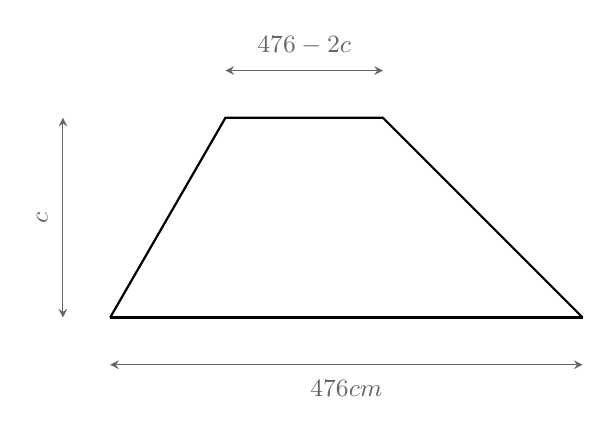
\begin{tikzpicture}[
    scale=2,
    cota/.style={<->, >=stealth, thin, gray!80!black},
    chamada/.style={gray!60, thin, dashed}
]
    % Coordenadas
    \coordinate (A) at (0, 0);
    \coordinate (B) at (3, 0);
    \coordinate (P1) at (0.732, 1.268);
    \coordinate (P2) at (1.732, 1.268);

    % Hachura do Engaste na base
    %\path[pattern={Lines[angle=45, distance=6pt, line width=0.5pt]}, pattern color=gray!60] (0, -0.3) rectangle (3, 0);

    % Desenho do Trapézio 4
    \draw[thick] (A) -- (B);                         % Borda engastada
    \draw[thick] (A) -- (P1) -- (P2) -- (B); % Linhas de charneira

    % Rótulo da Região
    %\node[font=\small\bfseries, gray!90!black, fill=white, inner sep=1.5pt, circle] at (1.232, 0.5) {4};

    % --- EIXO DE COTA HORIZONTAL INFERIOR (Base Maior - abaixo do engaste) ---
    \def\offsetHBaixo{0.3}
    %\draw[chamada] (A) -- (0, -\offsetHBaixo - 0.05);
    %\draw[chamada] (B) -- (3, -\offsetHBaixo - 0.05);
    \draw[cota] (0, -\offsetHBaixo) -- (3, -\offsetHBaixo)
        node[midway, below=2pt, font=\small] {$476\text{ cm}$};

    % --- EIXOS DE COTA HORIZONTAIS SUPERIORES (Base Menor e Projeções) ---
    \def\offsetHTopo{0.3}
    \def\yCotaTopo{1.268 + \offsetHTopo}

    %\draw[chamada] (0, 0) -- (0, \yCotaTopo + 0.05);
    %\draw[chamada] (P1) -- (0.732, \yCotaTopo + 0.05);
    %\draw[chamada] (P2) -- (1.732, \yCotaTopo + 0.05);
    %\draw[chamada] (3, 0) -- (3, \yCotaTopo + 0.05);

    % Projeção esquerda
    %\draw[cota] (0, \yCotaTopo) -- (0.732, \yCotaTopo)
        %node[midway, above=2pt, font=\small] {$c$};

    % Base menor
    \draw[cota] (0.732, \yCotaTopo) -- (1.732, \yCotaTopo)
        node[midway, above=2pt, font=\small] {$476 - 2c$};

    % Projeção direita
    %\draw[cota] (1.732, \yCotaTopo) -- (3, \yCotaTopo)
        %node[midway, above=2pt, font=\small] {$c$};

    % --- EIXO DE COTA VERTICAL (Altura do Trapézio) ---
    \def\offsetV{0.3}
    %\draw[chamada] (A) -- (-\offsetV - 0.05, 0);
    %\draw[chamada] (0, 1.268) -- (-\offsetV - 0.05, 1.268);
    \draw[cota] (-\offsetV, 0) -- (-\offsetV, 1.268)
        node[midway, left=2pt, font=\small, rotate=90, anchor=south] {$c$};

\end{tikzpicture}